\chapter{O método dos elementos finitos}

\section{Introdução}
O método dos elementos finitos auxiliou muitos dos maiores desenvolvimentos industriais nos últimos anos e sua expansão está, em boa quantia, ligada ao avanço dos computadores modernos. Sua flexilidade e versatilidade são potencializadores de seu recente domínio no campo das análises computacionais. O método foi criado para a aplicação na mecânica dos sólidos, porém hoje é usado em aplicações diversas. Este trabalho está inserido na área originaria do método, por conseguinte a explicação será de forma canônica, desconsiderando as aplicações que fogem do escopo geral da mecânica dos sólidos. \\

\begin{comment}
"The limitations of the human mind are such that it cannot grasp the behavior of its
complex surroundings and creations in one operation." \cite{zienkiewicz2013}. \\

Os limites da mente humana são tais que ela não pode compreender o comportamento de seus complexos arredores e criações em uma única operação. Esta frase quer dizer que nem sequer entendemos nosso meio em apenas uma iteração, portanto não é esperado que consigamos replicar tais comportamentos em apenas uma iteração. 
\end{comment}
A divisão de tarefas complexas é uma prática comum em todos os campos do conhecimento. A linha de produção de automóveis exemplifica um processo complexo extremamente segmentado .\\ Um problema discreto é caracterizado por ser subdividido em porções finitas que compõe um inteiro bem definido. De acordo com \cite{zienkiewicz2013} este é o único tipo de problema que pode ser resolvidos por um computador. O ato de escrever um programa, que nada mais é do que uma lista de instruções a ser seguida, perpassa pela descrição do problema em pacotes de tamanho administrável. \\

Porém de acordo com \cite{zienkiewicz2013}, a formulação física e matemática da maioria dos problemas, que valem a pena ser resolvidos, forma um sistema contínuo que por sua vez é composto por porções ditas infinitesimais. Estes componentes são tão pequenos quanto devaneios permitirem, portanto formam um problema de dimensão infinita. Resolver um problema contínuo, é impossível a um computador, dado que isto implicaria seguir uma sequência infinita de instruções até o fim do problema. \\ 

A solução de sistemas contínuos faz uso de conceitos e manipulações matemáticas que levam à solução exata do problema, porém este tipo de solução infelizmente está limitada aos problemas de menor complexidade que não por isso são de menor importância. De acordo com \cite{zienkiewicz2013} para resolver problemas de maior complexidade são necessárias técnicas de discretização. Tais técnicas são responsáveis pela transformação de problemas contínuos em discretos. A consequência desta transformação é que a outrora solução exata torna-se uma aproximação. \\

A técnica de discretização mais usada no âmbito da mecânica dos sólidos é a dos elementos finitos. De acordo com \cite{zienkiewicz2013} não há uma data exata para especificar o dia e ano de sua criação. Porém, um dos primeiros artigos,  que usa o nome: Método dos Elementos Finitos, foi escrito por Ray Willian Clough em 1960, \cite{CloughFEA}. Muito embora Clough tenha sido um dos primeiros a dar nome ao método, ele não foi um dos primeiros a fazer contribuições significativas. Neste grupo estão: Lord Rayleigh, \cite{Rayleigh}, como um dos primeiros participantes falando sobre métodos variacionais. Boris Grigoryevich Galerkin,\cite{Galerkin}, criador do método de Galerkin e possivelmente um dos maiores contribuintes históricos para o método dos elementos finitos. A última grande contribuição vem do que provavelmente pode ser chamado de método irmão, que é o das diferenças finitas. \footnote{Algumas outras contribuições foram decisivas para se chegar no estado atual, porém  para uma leitura mais detalhada da criação do método cita-se ,\cite{zienkiewicz2013} Pg. 1-4, como uma fonte concisa e rápida da sua criação.} \\

Neste trabalho a técnica dos elementos finitos será apresentada sem considerar qualquer não linearidade. Não linearidades podem ser relacionadas ao material, quando um modelo não elástico é usado, à geometria, quando há contato ou grandes deslocamentos e/ou deformações e às cargas, quando são seguidoras. Esta apresentação simplificada é justificada pelo compartilhamento das bases formadoras do método em problemas lineares e não lineares.  \\

Em problemas envolvendo impacto balístico as não linearidades encontradas são relacionadas ao material e à geometria. No material a ocorrência de deformações plásticas insere a necessidade de modelos constitutivos não lineares. Quanto à geometria, grandes deslocamentos e deformações estão presentes neste tipo de evento, portanto há necessidade de usar o tensor de deformações finitesimais para sua descrição. \\ 

Como dito anteriormente as não linearidades serãoo desconsideradas, portanto as deformações serão consideradas infinitesimais. Além disso, os efeitos da temperatura não serão levados em consideração. Como apresentado no \ref{Cap:MecCont} a expressão \ref{eq:locallinbal} é a forma local do balanço de momento linear, também chamada de primeira equação do movimento de Cauchy. Doravante os dois nomes serão usados. Já que tudo que vem a seguir será apresentado considerando deformações infinitesimais não haverá distinção entre a configuração material e espacial. 

\section{Condições iniciais e de contorno}

O objetivo é resolver a forma local do balanço de momento linear. A forma do balanço de momento adequada resolução é obtida notando que $ \dot{\boldsymbol{v}}(\boldsymbol{x},t) = \ddot{\boldsymbol{u}}(\boldsymbol{x},t) $ onde $ \boldsymbol{u} = \boldsymbol{u}(\boldsymbol{x},t)$ é o campo dos deslocamentos e $ \ddot{\boldsymbol{u}} = \ddot{\boldsymbol{u}} (\boldsymbol{x},t) $ é o campo das acelerações. A forma a ser resolvida está na expressão \ref{eq:balancoresolvido} \\ A resolução feita em função do campo de deslocamentos gera um problema de valor inicial de segunda ordem, no qual são necessárias duas condições iniciais e duas de contorno.\\

\begin{equation}\label{eq:balancoresolvido}
	div\boldsymbol{\sigma(\boldsymbol{u})} + \boldsymbol{b} = \rho \ddot{\boldsymbol{u}}
\end{equation}

As condições iniciais são o deslocamento e a velocidade em $ t = 0 $, que podem ser denotadas da seguinte forma.

\begin{align} 
	\boldsymbol{u}(\boldsymbol{x},t)|_{t=0} = \boldsymbol{u}_{0}(\boldsymbol{x}) \\
	\dot{\boldsymbol{u}}(\boldsymbol{x},t)|_{t=0} = \dot{\boldsymbol{u}_{0}}(\boldsymbol{x})
\end{align} 

As condições de contorno são aplicadas no ou nos contornos do corpo. Observa-se na figura \ref{fig:condcont}, que há distinção entre duas regiões do contorno. A primeira região a ser considerada é $ \partial \Omega_u $, onde são aplicadas as condições de contorno essenciais ou de Dirichlet. Conforme \cite{Paulo} estas condições são responsáveis pela restrição dos movimentos de corpo rígido. Na figura \ref{fig:condcont} é apresentado um corpo em duas dimensões, portanto este tem três movimentos de corpo rígido. Estes devem ser restritos para a solução de um problema estático hipotético. Em um problema dinâmico os movimentos de corpo rígido só devem ser restritos quando necessário para a correta representação da situação simulada. De acordo com \cite{Paulo} estas condições de contorno são chamadas de essenciais pois restringem a variável primal do problema, $ \boldsymbol{u}(\boldsymbol{x},t) $ neste caso. Sua representação é feita da seguinte forma.

\begin{equation}
	u = \overline{u} \quad \forall \; \boldsymbol{x} \; \in  \partial \Omega_u
\end{equation}

Onde \gls{u} é o campo vetorial de deslocamentos do corpo. Uma consideração a ser feita é o impacto numérico das condições de contorno essenciais. O método dos elementos finitos resulta em uma equação algébrica a ser resolvida. No caso de sistemas mecânicos estáticos e lineares a seguinte equação algébrica é o resultado do método:
\begin{equation}
    \boldsymbol{K} \boldsymbol{U} = \boldsymbol{F} 
\end{equation}
$ \boldsymbol{K} $ chama-se matriz de rigidez. Caso não sejam aplicadas condições de contorno essenciais, em um problema estático, ela é singular. Um sistema contendo uma matriz singular não tem uma solução unívoca, portanto não é útil. O Fato de não ter solução unívoca tem leitura física imediata: Sem as condições de contorno essenciais o corpo tem seus movimentos de corpo rígido irrestritos, então infinitos campos de deslocamento podem ser responsáveis pela mesma deformação. A matriz $\boldsymbol{K} $ passa a ser não singular, o sistema passa a ter solução univoca, quando as condições de contorno essenciais são bem postas. Condições bem postas são, neste caso, aquelas que restringem todos os movimentos de corpo rígido em um sistema estático. Em sistemas dinâmicos as forças de d'Alembert se contrapõem ao movimento irrestrito, de acordo com \cite{Paulo}. Mesmo sem o problema da singularidade estar presente, as condições de contorno são extremamente importantes para a correta tradução da física do fenômeno.\footnote{Por tradução quer-se dizer transferência do fenômeno para um problema numérico. O prof. Paulo de tarso Rocha de Mendonça, autor de \cite{Paulo} disse em uma de suas aulas que é comum resolver corretamente o problema errado. } \\

\begin{figure}
	\caption{Corpo com condições de contorno.}
	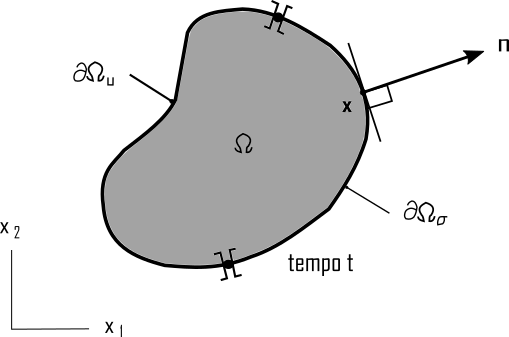
\includegraphics{images/CorpoCondCont.png}
	\label{fig:condcont}
	\fonte{O autor (2020)}
\end{figure}

As condições de contorno naturais ou condições de contorno de Von Neumann são identificadas fisicamente como trações de superfície. Elas são necessárias para a correta descrição do problema diferencial, sendo responsáveis pelas forças aplicadas ao corpo. Estas condições não atuam na variável primal. Elas atuam no campo de tensões, que é função do campo de deslocamentos através da relação ou modelo constitutivo usado. As condições de contorno naturais podem ser descritas da seguinte forma.

\begin{equation}
	\boldsymbol{t} = \boldsymbol{\sigma}\boldsymbol{n} = \boldsymbol{\overline{t}} \quad \forall \; \boldsymbol{x} \; \in \; \partial \Omega_{\sigma}
\end{equation}

Agora todas as expressões necessárias para uma definição bem posta de um problema diferencial estão disponíveis. De acordo com \cite{Paulo} neste estado o problema está na forma chamada forte, pois fornece a solução exata restringindo as possíveis soluções ao conjunto de funções $C1$. \footnote{Conjunto de funções onde, além de outras exigências, a primeira derivada deve ser contínua.} O problema a ser resolvido na forma forte é o seguinte:
\begin{align}
    \begin{cases}
	div\boldsymbol{\sigma(\boldsymbol{u})} + \boldsymbol{b} = \rho \ddot{\boldsymbol{u}}\\
	u = \overline{u} \quad \forall \; \boldsymbol{x} \; \in  \partial \Omega_u\\
	\boldsymbol{t} = \boldsymbol{\sigma}\boldsymbol{n} = \boldsymbol{\overline{t}} \quad \forall \; \boldsymbol{x} \; \in \; \partial \Omega_{\sigma} \\
	\boldsymbol{u}(\boldsymbol{x},t)|_{t=0} = \boldsymbol{u}_{0}(\boldsymbol{x}) \\
	\dot{\boldsymbol{u}}(\boldsymbol{x},t)|_{t=0} = \dot{\boldsymbol{u}_{0}}(\boldsymbol{x})
	\end{cases}
\end{align}

A solução de um problema na forma forte deve ser obtida através de procedimentos analíticos, já que este é contínuo. Por conta disto, a resolução deste problema em domínios arbitrários não é trivial. De acordo com \cite{Paulo} a forma forte deve ser transformada em uma forma chamada fraca, para então ser discretizada e resolvida numericamente.

\subsection{A forma fraca}
A construção da forma fraca será feita pelo principio dos trabalhos virtuais, conhecido como PTV. O primeiro passo para tal é multiplicar a equação por uma função vetorial arbitrária, que é representada por $ \boldsymbol{\hat{u}} = \boldsymbol{\hat{u}}(\boldsymbol{x})  $ e é chamada função teste ou de deslocamentos virtuais. Ao integrar, ao longo de todo o corpo, o resultado da operação anterior é obtida a equação \ref{eq:formafraca1}.
\begin{equation}
\int_{\Omega} div(\boldsymbol{\sigma}) \cdot \boldsymbol{\hat{u}} + \boldsymbol{b} \cdot \boldsymbol{\hat{u}} - \rho\ddot{\boldsymbol{u}} \cdot \boldsymbol{\hat{u}} \; dV = 0
\label{eq:formafraca1}
\end{equation}

De acordo com \cite{Holzapfel} o próximo passo é aplicar a regra do produto, usando a simetria do tensor de tensões de Cauchy. Com isso, é possível trabalhar o primeiro termo da integral em \ref{eq:formafraca1} da seguinte forma.\footnote{Esta passagem não é trivial, porém a expressão da regra do produto usada pode ser encontrada sem derivação em \cite{Holzapfel} equação 1.290}
\begin{equation}
	div \boldsymbol{\sigma} \cdot \boldsymbol{\hat{u}} = div(\boldsymbol{\sigma}\boldsymbol{\hat{u}}) - \boldsymbol{\sigma} : grad \boldsymbol{\hat{u}}
	\label{eq:formafraca2}
\end{equation}

Ao aplicar o teorema do divergente, a propriedade comutativa do produto interno e novamente a simetria do tensor de tensões de Cauchy no primeiro termo do braço direito da equação \ref{eq:formafraca2}. Obtêm-se a seguinte expressão.
\begin{equation} \label{eq:formafracatrans}
	\int_{\Omega} div(\boldsymbol{\sigma \hat{u}}) dV = \int_{\partial \Omega} \boldsymbol{\sigma \hat{u}} \cdot \boldsymbol{n} ds = \int_{\partial \Omega} \boldsymbol{\sigma n} \cdot \boldsymbol{\hat{u}} ds
\end{equation}

Ao substituir \ref{eq:formafracatrans} na equação \ref{eq:formafraca1}, é obtida a seguinte expressão.

\begin{equation}
\int_{\Omega} \boldsymbol{\sigma} : grad \boldsymbol{\hat{u}} -  \boldsymbol{b} \cdot \boldsymbol{\hat{u}} + \rho\ddot{\boldsymbol{u}} \cdot \boldsymbol{\hat{u}} dV - \int_{\partial \Omega} \boldsymbol{\sigma n} \cdot \boldsymbol{\hat{u}} ds = 0
\label{eq:formafraca3}
\end{equation}

Para continuar a derivação é necessária uma discussão sobre \gls{u} e \gls{uvir}.  Assim como aponta \cite{Paulo} o campo de deslocamentos pertence ao conjunto de funções cinematicamente admissíveis, definido por 
\begin{equation}
	Kin = \{ \boldsymbol{u}(\boldsymbol{x},t) \; é \; suficientemente \; regular \; tal \; que \; \boldsymbol{u}(\boldsymbol{x},t) = \boldsymbol{\overline{u}}  \quad \forall \boldsymbol{x} \in \partial \Omega_u \}
\end{equation}

Já os deslocamentos virtuais chamados anteriormente de arbitrários devem pertencer ao chamado espaço das variações.
\begin{equation}
	Var  = \{ \boldsymbol{\hat{u}}(\boldsymbol{x}) \; é \; suficientemente \; regular \; tal \; que \; \boldsymbol{\hat{u}}(\boldsymbol{x}) = 0  \quad \forall \boldsymbol{x} \in \partial \Omega_u \}
\end{equation}


De acordo com \cite{Paulo} agora ao destaca-se a segunda integral da equação \ref{eq:formafraca3}, considerando que $ \boldsymbol{\overline{u}} = 0 \quad \forall \boldsymbol{x} \in \partial \Omega_u $ e sabendo que $ \boldsymbol{\sigma n} = \boldsymbol{\overline{t}} \quad \forall \in \partial \Omega_{\sigma} $.

\begin{equation} \label{eq:formafracatrans}
	\int_{\partial \Omega} \boldsymbol{\sigma n} \cdot \boldsymbol{\hat{u}} ds = \int_{\partial \Omega_u} \boldsymbol{\sigma n} \cdot \boldsymbol{0} ds + \int_{\partial \Omega_{\sigma}} \boldsymbol{\overline{t}} \cdot \boldsymbol{\hat{u}} ds = \int_{\partial \Omega_{\sigma}} \boldsymbol{\overline{t}} \cdot \boldsymbol{\hat{u}} ds 
\end{equation}

A forma fraca do problema é finalmente caracterizada pela seguinte expressão, onde \ref{eq:formafracatrans} foi inserido em \ref{eq:formafraca3}.

\begin{equation} \label{eq:formafracafinal}
	\int_{\Omega} \boldsymbol{\sigma} : grad \boldsymbol{\hat{u}} -  \boldsymbol{b} \cdot \boldsymbol{\hat{u}} +  \rho\ddot{\boldsymbol{u}} \cdot \boldsymbol{\hat{u}}  dV - \int_{\partial \Omega_{\sigma}} \boldsymbol{\overline{t}} \cdot \boldsymbol{\hat{u}} ds = 0 
\end{equation}

De acordo com \cite{Paulo} a função de teste $ \hat{u} $ tem um significado especial no principio dos trabalhos virtuais. Ela é chamada de deslocamentos virtuais e forma trabalhos virtuais quando associada às forças internas e externas. A identificação dos termos da forma fraca, de acordo com o princípio dos trabalhos virtuais, é feita a seguir.
\begin{itemize}
	\item Trabalho virtual interno
	\begin{equation}
		\int_{\Omega} \boldsymbol{\sigma} : grad\boldsymbol{\hat{u}} dV
	\end{equation}
	\item Trabalho virtual externo
	\begin{equation}
		\int_{\Omega} \boldsymbol{b} \cdot \boldsymbol{\hat{u}} dV + \int_{\partial \Omega_{\sigma}} \boldsymbol{\overline{t}} \cdot \boldsymbol{\hat{u}} d\partial \Omega_{\sigma}
	\end{equation}
	\item Termo relacionado à inercia
	\begin{equation}
		\int_{\Omega} \rho \ddot{\boldsymbol{u}} \cdot \boldsymbol{\hat{u}}  dV
	\end{equation}
\end{itemize}

Antes de partir para a solução da forma fraca, é preciso esclarecer se ela é válida para resolver a forma forte. Pelo lema fundamental do cálculo variacional:\\
Dada uma função $ f(x) $ contínua, se
\begin{equation}
\int_{a}^{b} f(x) h(x) dx = 0
\end{equation}
para toda e qualquer função arbitrária $ h(x) $,
então $ f(x) = 0 $ no intervalo (a,b). \\

A partir de \ref{eq:formafraca1}, reduzindo a equação para a forma unidimensional, é evidenciado que o lema fundamental apresentado acima evidencia que a forma forte é resolvida pela forma fraca.
\begin{align}
	\int_{\Omega} \frac{\partial \sigma_x}{\partial x} \hat{u} + b_x \hat{u} - \rho\ddot{u} \hat{u} \; dx = 0 \\
	\int_{\Omega} (\frac{\partial \sigma_x}{\partial x}  + b_x - \rho\ddot{u} )\hat{u} \; dx = 0
\end{align}

\subsection{A Discretização no espaço}

Para resolver a forma fraca é necessário discretizar o domínio no espaço. A descrição em uma dimensão será usada, todavia os conceitos apresentados são iguais independente de quantas dimensões são empregadas. O domínio representado pelo conjunto (a,b) é contínuo, portanto de acordo com \cite{Paulo} tem dimensão infinita. Este deve ser dividido em regiões menores, de forma que.
\begin{equation} \label{eq:malha1d}
	x_1 = a \quad x_i<x_{i+1} \quad e \; x_N = b
\end{equation}

Em uma dimensão cada intervalo de $ x_i $  a $ x_{i+1} $ define um elemento do domínio. A soma de todos os elementos, em conjunto com o contorno, compõe o domínio do problema que agora é finito. Os pontos $ x_i $ são chamados de nós, e a união entre elementos e nós forma uma malha. \\

A aproximação das funções $ u(x,t) \; e \; \hat{u}(x,t) $ é feita da seguinte maneira.
\begin{align} 
	u(x,t) \approx u_h(x,t) = \sum_{n=1}^{N} \phi_n (x) u_n(t) \\
	\hat{u}(x,t) \approx \hat{u}_h(x) = \sum_{m=1}^{N} \phi_m (x) \hat{u}_m  
\end{align}

Onde $ u_n $ e $ \hat{u}_m $ são valores nodais dos respectivos campos.
De acordo com \cite{zienkiewicz2013} considerando a malha expressa por \ref{eq:malha1d}, é possível definir o conjunto de funções polinomiais de aproximação a seguir.

\begin{equation} \label{eq:funcform}
    \phi_i =  \left \{ \begin{array}{rcl}
         0, & \text{se} & x < x_{i-1} \\
        \ddfrac{x - x_{i-1}}{x_i - x_{i-1}}, &  \text{se} & x_{i-1} < x < x_{i} \\
        \ddfrac{x_{i+1} - x}{x_{i+1} - x_{i}}, &  \text{se} & x_i < x < x_{i+1} \\
         0, & \text{se} & x > x_{i+1}
    \end{array} \right.
\end{equation}

\begin{figure}[h] % TODO: Inserir fonte \cite{zienc}
    \centering
    \caption{ a: Funções de aproximação descritas em \ref{eq:funcform}. b: Derivadas das mesmas funções }
    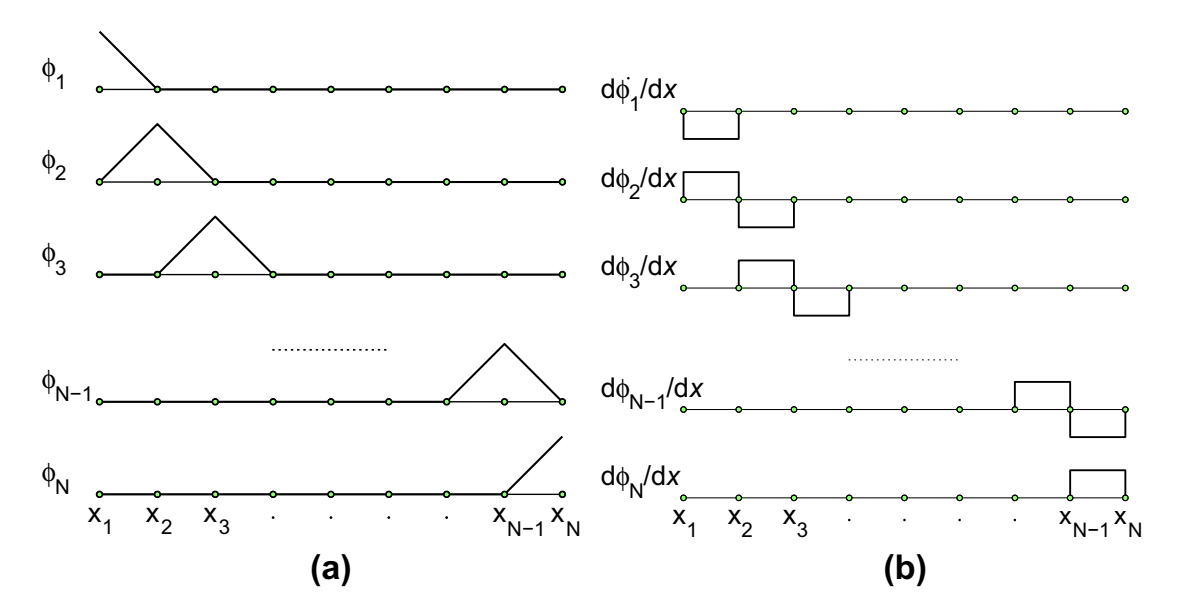
\includegraphics[width=0.8\linewidth]{images/funcform.png}
    \label{fig:funcform}
    \fonte{\cite{zienkiewicz2013}}
\end{figure}

A figura \ref{fig:funcform} mostra as funções definidas em \ref{eq:funcform}. De acordo com \cite{zienkiewicz2013} estas funções são pertencentes ao conjunto $C0$, portanto são simplesmente contínuas. Sendo assim, suas derivadas são apenas contínuas por partes.

De acordo com \cite{zienkiewicz2013}. ao considerar que o modelo constitutivo é a lei de Hooke, que o corpo tem coeficiente de Poisson nulo e que cargas superficiais não estão presentes. A forma fraca unidimensional é descrita da seguinte forma.\footnote{Considerar Poisson nulo, neste caso, permite que exista apenas a componente $ \sigma_x $} \footnote{De acordo com a lei de Hooke $ \sigma_x = E \varepsilon_x = E \frac{\partial u}{ \partial x} $}
\begin{equation} \label{eq:formafracalin}
    \int_{\Omega} \hat{u} (\rho \ddfrac{\partial^2 u}{\partial t^2} - b_x) \, dx + \int_{\Omega} \ddfrac{\partial \hat{u}}{\partial x} E \ddfrac{\partial u}{ \partial x} \,  dx
\end{equation}

De acordo com \cite{zienkiewicz2013}  as integrais no domínio do corpo podem ser computadas da seguinte forma

\begin{equation} \label{eq:integraisdif}
    \int_{\Omega} (\cdot) \, dx = \sum_{i = 1}^{N_{el}} \int_{x_i}^{x_{i+1}} (\cdot) \, dx \equiv \sum_{e} \int_{\Omega_e} (\cdot) dx
\end{equation}

Onde $ N_{el} $ é o número de elementos, e $\sum_e$ é um somatório que compreende todos os elementos. A última integral em \ref{eq:integraisdif} mostra que é possível calcular a participação de cada elemento, desta forma a integral no domínio é a soma das participações dos elementos. O criador de um dos maiores softwares de código aberto em elementos finitos, autor de  \cite{BangerthHartmannKanschat2007}, afirma em uma de suas videoaulas que a capacidade de tratar de forma igualitária cada elemento é uma das maiores vantagens computacionais do método dos elementos finitos.\footnote{O sitio para acesso das videoaulas é \url{https://www.math.colostate.edu/~bangerth/videos.html}} \\

\begin{figure}
    \centering
    \caption{a: Funções de forma para um certo elemento. b: Derivadas das mesmas funções}
    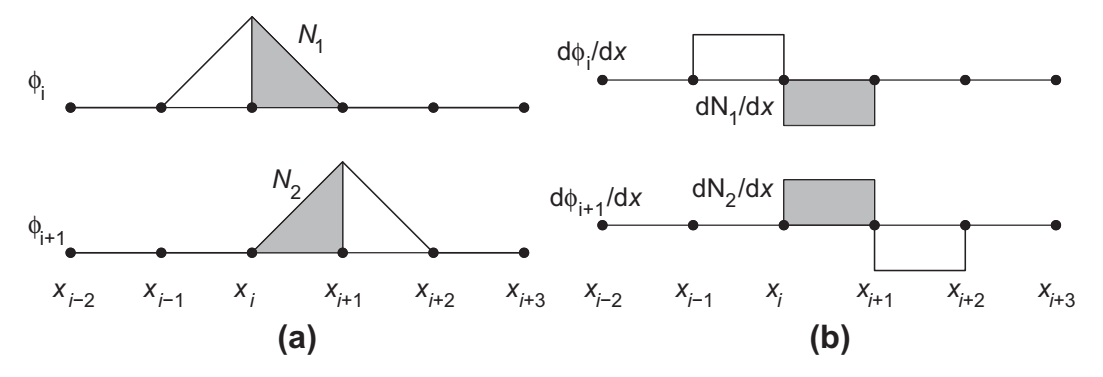
\includegraphics[width=0.8\linewidth]{images/funcformaverdade.png}
    \label{fig:funcformverd}
    \fonte{\cite{zienkiewicz2013}}
\end{figure}

De acordo com \cite{zienkiewicz2013} todos os elementos ou intervalos $ [x_i, x_{i+1}] $ presentes na figura \ref{fig:funcformverd} usam as mesmas funções $ N_1 $  e $ N_2 $ para sua definição, portanto estas são chamadas funções de forma para o elemento. Um elemento é chamado de linear ou quadrático quando suas funções de forma são lineares ou quadráticas e assim por diante. As seguintes propriedades são válidas e necessárias para as funções de aproximação, que dentro de um elemento são chamadas de função de forma, de acordo com \cite{Paulo}.

\begin{itemize}
    \item Uma função associada a um certo nó $ i $ é nula em todos os outros nós da malha.
    \item Cada função $ \phi_i $ é nula em todos os elementos que não contém o nó $i$.
    \item A soma de todas as funções de aproximação em um ponto qualquer é \begin{equation}
        \sum^N_{n=i} \phi_n (x) = 1
    \end{equation} um conjunto de funções que satisfazem essa propriedade são ditas partição da unidade. 
\end{itemize}

Dado que a integral é feita em cada elemento  um sistema de coordenadas locais é inserido, nele
\begin{equation}
    x' =  x - x^e_1 
\end{equation}

na qual $ x^e_1 $ é a coordenada do primeiro nó de um elemento $e $, $x$ é a coordenada global e $x'$ a coordenada local. De acordo com \cite{zienkiewicz2013}, ao aplicar o sistema de coordenadas local nas funções de forma. As aproximações dos campos de deslocamento e de deslocamento virtual são escritas da seguinte maneira

\begin{align}
    u_h^e = N_1(x')u_1^e + N_2(x')u_2^e \\
    \hat{u}_h^e = N_1(x')\hat{u}_1^e + N_2(x')\hat{u}_2^e
\end{align}

Onde $ u^e_i $ e $ \hat{u}^e_i $ é a aproximação do respectivo campo $ u $ ou $ \hat{u} $ no nó $ i $ do elemento $ e $. Ao aplicar estas aproximações na forma fraca apresentada em \ref{eq:formafracalin}, seguida da separação dos termos de acordo com sua contribuição energética. De acordo com \cite{zienkiewicz2013}, são formadas as seguintes expressões

\begin{itemize}
    \item Termo relacionado à inercia: \begin{equation}
        \sum_{e=1}^M [\hat{u}^e_1 \, \hat{u}^e_2 ] \int_{\Omega_e} \begin{Bmatrix} N_1 \\ N_2 \end{Bmatrix} \rho \begin{Bmatrix} N_1 & N_2 \end{Bmatrix} \; dx' \begin{Bmatrix} \ddot{u}^e_1 \\ \ddot{u}^e_2 \end{Bmatrix}
    \end{equation}
    
    \item Termo relacionado à tensão interna \begin{equation}
        \sum_{e=1}^M [\hat{u}^e_1 \, \hat{u}^e_2 ] \int_{\Omega_e} \begin{Bmatrix} \ddfrac{dN_1}{dx'} \\ \ddfrac{dN_2}{dx'}  \end{Bmatrix} E \begin{Bmatrix} \ddfrac{dN_1}{dx'}  & \ddfrac{dN_2}{dx'}  \end{Bmatrix} \; dx' \begin{Bmatrix} u^e_1 \\ u^e_2 \end{Bmatrix}
    \end{equation}
    
    \item Termo relacionado às forças de corpo: 
    \begin{equation}
        \sum_{e=1}^M [\hat{u}^e_1 \, \hat{u}^e_2 ] \int_{\Omega_e} \begin{Bmatrix} N_1 \\ N_2  \end{Bmatrix} b_x \; dx'
    \end{equation}
\end{itemize}

Avaliando as integrais dos termos acima são obtidas matrizes e vetores pertencentes ao elemento $e$. Computar as integrais apresentadas aqui é trivial, já que as expressões foram extremamente simplificadas. Em um problema com duas ou três dimensões calcular analiticamente as integrais formadas não é factível. De acordo com \cite{zienkiewicz2013} o cálculo das integrais frmadas é feito usando integrações numéricas chamadas de quadraturas.\footnote{A quadratura mais usada é a de Gauss-Legendre, explicações sobre as quadraturas e suas peculiaridades são encontradas em \cite{Paulo} e \cite{zienkiewicz2013}} As matrizes de massa e rigidez, assim como o vetor de forças de corpo são resultados do cálculo das integrais previamente citadas. 

\begin{itemize}
    \item Matriz de massa do elemento : \begin{equation} \boldsymbol{M}^e = \int_{\Omega_e} \begin{Bmatrix} N_1 \\ N_2 \end{Bmatrix} \rho \begin{Bmatrix} N_1 & N_2 \end{Bmatrix} \; dx' = \begin{bmatrix} M^e_{11} & M^e_{12} \\ M^e_{21} & M^e_{22} \end{bmatrix} \end{equation} 
    \item Matriz de rigidez do elemento: \begin{equation}
        \boldsymbol{K}^e = \int_{\Omega_e} \begin{Bmatrix} \ddfrac{dN_1}{dx'} \\ \ddfrac{dN_2}{dx'}  \end{Bmatrix} E \begin{Bmatrix} \ddfrac{dN_1}{dx'}  & \ddfrac{dN_2}{dx'}  \end{Bmatrix} \; dx' = \begin{bmatrix} K^e_{11} & K^e_{12} \\ K^e_{21} & K^e_{22} \end{bmatrix}
    \end{equation}
    
    \item Vetor de forças de corpo do elemento: 
    \begin{equation}
        \boldsymbol{F}^e = \int_{\Omega_e} \begin{Bmatrix} N_1 \\ N_2  \end{Bmatrix} b_x \; dx' = \begin{bmatrix} F^e_1 \\ F^e_2 \end{bmatrix}
    \end{equation}
\end{itemize}

 De acordo com \cite{Paulo} ao considerar que  $ \hat{u} \neq 0 $, além disso somando todas as participações dos elementos. O sistema torna-se uma equação algébrica, vide equação \ref{eq:formafindiscesp}.

\begin{equation} \label{eq:formafindiscesp}
    \boldsymbol{M \ddot{u} } + \boldsymbol{Ku} = \boldsymbol{F}
\end{equation}

Sendo $ \boldsymbol{M} $ e $ \boldsymbol{K} $ as matrizes de massa e rigidez, $\boldsymbol{F}$ o vetor de forças de corpo, $ \boldsymbol{\ddot{u}} $ o vetor das acelerações nodais e $\boldsymbol{u}$ o vetor de deslocamentos nodais.\\

A equação algébrica \ref{eq:formafindiscesp} é a forma final da discretização espacial de um sistema linear.

\subsubsection{A discretização de um problema dinâmico}

A discretização de um problema dinâmico tem algumas particularidades a serem consideradas. Uma delas é chamada de trancamento ou em inglês "Locking". De acordo com \cite{Paulo} o trancamento é observado em elementos lineares contendo todos os pontos de integração, estes pontos são oriundos da integração numérica usada na solução. O trancamento se manifesta através de um excesso de rigidez na malha, por conseguinte os deslocamentos são subestimados e o resultado é fisicamente inválido. \\

A técnica de integração numérica mais usada é a quadratura de Gauss-Legendre. Um polinômio de grau $p$ necessita de $np$ pontos em sua integração para ser integrado de forma exata, de acordo com a equação \ref{eq:quadratu}. 
\begin{equation} \label{eq:quadratu}
    P=2np-3
\end{equation}

De acordo com \cite{Paulo} são necessários oito pontos para integrar exatamente um elemento hexaédrico de oito nós, representado na figura \ref{fig:hexaoito}. Este elemento usa funções lineares semelhantes às funções apresentadas no exemplo unidimensional, porém sua dimensão faz com que estejam presentes funções de grau 2 na integral do elemento. Os pontos de integração estão representados na figura  \ref{fig:hexapontos}. \\
\begin{figure}
\caption{Elemento hexaédrico de oito nós e seus pontos de integração.}

\begin{subfigure}{0.5\textwidth}
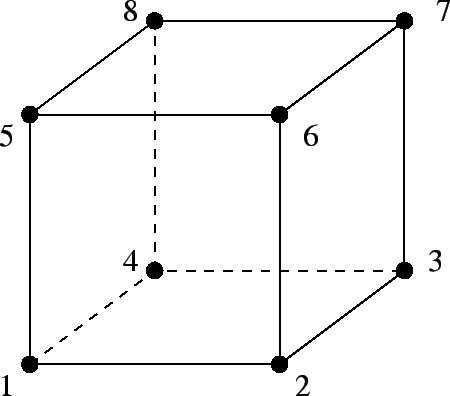
\includegraphics[width=0.9\linewidth, height=5cm]{images/hexapointsofint.png}
    \caption{Elemento hexaédrico de oito nós}
    \label{fig:hexaoito}
\end{subfigure}
\begin{subfigure}{0.5\textwidth}
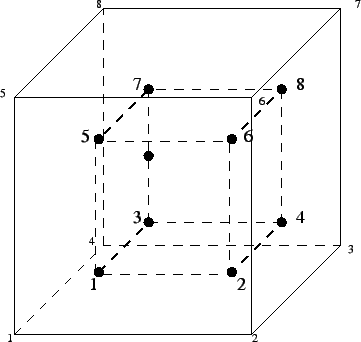
\includegraphics[width=0.9\linewidth, height=5cm]{images/hexaelement.png}
\caption{Pontos de integração do elemento}
\label{fig:hexapontos}
\end{subfigure}
\label{fig:hexaele}

\fonte{ \url{http://web.mit.edu/calculix_v2.7/CalculiX/ccx_2.7/doc/ccx/node26.html}}
\end{figure}
%CONTINUAR REVISAO%

A integração completa, ou seja integrar usando todos os pontos provenientes da quadratura, de elementos lineares pode gerar trancamento. Além disso, o custo computacional deste tipo de integração é extremamente alto, dado que malhas com elementos muito pequenos são necessárias para a correta solução de um problema de impacto balístico. A solução encontrada é uma técnica chamada subintegração. Ela consiste em usar menos pontos de integração do que seriam necessários para o elemento. No caso dinâmico é costumeiro usar apenas um ponto e este é localizado no centro do elemento. De acordo com \cite{theorymanls} os elementos com um ponto de integração são 25 vezes menos custosos em termos computacionais, em relação aos totalmente integrados. Embora a subintegração diminua o custo computacional e resolva o trancamento ela não é a solução perfeita, já que este tipo de técnica tem problemas colaterais associados a seu uso. \par

Os problemas gerados pela subintegação são a representação da tensão como um tensor constante no elemento e o surgimento de modos espúrios de deformação. A representação da tensão como constante não é um grande problema, já que um refino de malha é suficiente para sua solução. Os modos espúrios de deformação causam muito mais dor de cabeça ao analista. O que acontece é que os elementos se deformam sem gastar energia e com isso geram ruídos na energia total do sistema, portanto é necessário controla-los. Estes modos espúrios de deformação são chamados de ampulheta ou "Hourglass". O nome ampulheta se dá por conta do formato assumido pelo conjunto de dois elementos quando estão se deformando em modo espúrio, vide figura \ref{fig:hourglass}. 

\begin{figure}
    \centering
    \caption{Deformação espúria formando uma ampulheta entre os elementos.}
    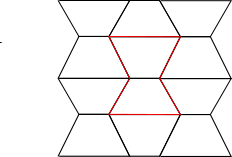
\includegraphics[width=0.5\linewidth]{images/hourglass.png}
    \label{fig:hourglass}
    \fonte{O autor (2020)}
\end{figure}

\subsection{A discretização no tempo}

A equação algébrica \ref{eq:formafindiscesp} está discretizada no espaço, porém note que não foi feita qualquer consideração quanto ao tempo. É necessário discretizar esta equação no tempo e isso é feito usando um método de marcha. De acordo com \cite{Paulo} este nome vem do fato de que o tempo é subdividido em intervalos e um algoritmo passa por cada um deles de forma sequencial. O intervalo de tempo considerado é $[t_0,t_f] $ . A marcha ocorrerá de forma a passar por um intervalo $ \Delta t $ a cada iteração, sendo $ t_1 = t_0 + \Delta t $, $ t_2 = t_0 + 2 \Delta t = t_1 + \Delta t $ e assim por conseguinte. Existem dois grupos de métodos usados para realizar esta marcha no tempo, são eles implícitos e explícitos. \\

A escolha entre os métodos leva em consideração o comportamento esperado da solução, que pode ser classificado de acordo com o formato da equação diferencial resolvida. De acordo com \cite{BangerthHartmannKanschat2007} a equação de onda é classificada como hiperbólica, logo não é esperada a atenuação da curva descrita pela variável essencial. Um impacto em alta velocidade excita frequências altas dos corpos envolvidos, assim é necessário que o passo de tempo seja pequeno para que as influências destas faixas de frequência sejam corretamente computadas. O custo computacional de cada $\Delta t$ em um método implícito é muito mais alto do que em um método explícito, no entanto estes métodos são incondicionalmente estáveis. Dizer que o método é incondicionalmente estável significa que é possível usar passos de tempo tão grandes quanto desejado. Em um método condicionalmente estável há uma limitação quanto ao passo usado, nestes é preciso reduzir o $ \Delta t $ de acordo com a equação \ref{eq:defdeltat}. Onde $l$ é a menor dimensão de um elemento da malha, $c$ é a velocidade do som no material e $k$ é um fator de estabilidade que normalmente varia entre 0.6 e 0.9. \\


Para o caso de impactos balísticos, que envolvem velocidades relativamente altas, os métodos explícitos são mais interessantes. Conforme \cite{Zukas} o uso de grandes passos de tempo faz com que detalhes da solução sejam perdidos, logo não seria possível extrair benefício da estabilidade incondicional dos métodos implícitos e métodos explícitos são preferidos por seu custo inferior. \\

\begin{equation}
\Delta t = \frac{k l }{c}
\label{eq:defdeltat}
\end{equation}

A equação \ref{eq:formafindiscesp} é escrita da seguinte forma
    \begin{equation} \label{eq:formainicialdisctempo}
    \boldsymbol{M \ddot{u}_n } + \boldsymbol{K}\boldsymbol{u}_n = \boldsymbol{F}_n
\end{equation}
Onde $ u_n $ é o deslocamento em $t=n$, portanto a equação \ref{eq:formainicialdisctempo} descreve o sistema em um determinado tempo $t_n $. È necessário que todos os valores sejam conhecidos em e até $ t_n $. As condições iniciais são usadas para caracterizar o sistema em $ t_0 $. Para avançar no tempo o método das diferenças centrais toma a velocidade média em cada intervalo da seguinte forma

\begin{align} \label{eq:vels}
    \dot{u}_{n-\frac{1}{2}} \approx \ddfrac{u_n - u_{n-1}}{\Delta t} & \hspace{25mm} \text{e} & \dot{u}_{n+\frac{1}{2}} \approx \ddfrac{ u_{n+1} + u_n}{\Delta t} 
\end{align} 

Usando as velocidades definidas em \ref{eq:vels} é possível escrever a aceleração $ \ddot{u}_n $ 

\begin{equation} \label{eq:acels}
    \ddot{u} = \ddfrac{u_{n+1} - 2u_n + u_{n-1}}{\Delta t^2}
\end{equation}

Agora substituindo \ref{eq:acels} em \ref{eq:formainicialdisctempo} a seguinte expressão é alcançada.

\begin{equation} \label{eq:formaquasefimdisctempo}
    \ddfrac{1}{\Delta t^2}\boldsymbol{M} \boldsymbol{u_{n+1}} = [\boldsymbol{F}_n - \boldsymbol{Ku}_n + \ddfrac{1}{\Delta t^2}\boldsymbol{M}(2\boldsymbol{u}_n - \boldsymbol{u}_{n-1}) ]
\end{equation}

Para transformar \ref{eq:formaquasefimdisctempo} em sua forma explícita é necessário realizar o procedimento de diagonalização da matriz de massa, que faz com que todos os termos sejam transferidos para a diagonal principal. De acordo com \cite{Paulo} este procedimento implica perda de informação, o que gera erros adicionais de aproximação. Porém para que o procedimento de diagonalização seja válido se faz necessário que a massa de cada elemento seja conservada. Depois da diagonalização a equação \ref{eq:formaquasefimdisctempo} assume sua forma final e por sua vez explícita, já que de acordo com \cite{Paulo} não há necessidade de se resolver um sistema algébrico.

\begin{equation}
    u^j_{n+1} = (\ddfrac{M_{jj}}{\Delta t^2} )^-1 [F_n^j - (Ku_n)^j + \ddfrac{1}{\Delta t^2}M_{jj}(2u_n^j - u_{n-1}^j) + \ddfrac{1}{2 \Delta t}C u_{n-1}]
\end{equation}

